% This file was created with tikzplotlib v0.10.1.
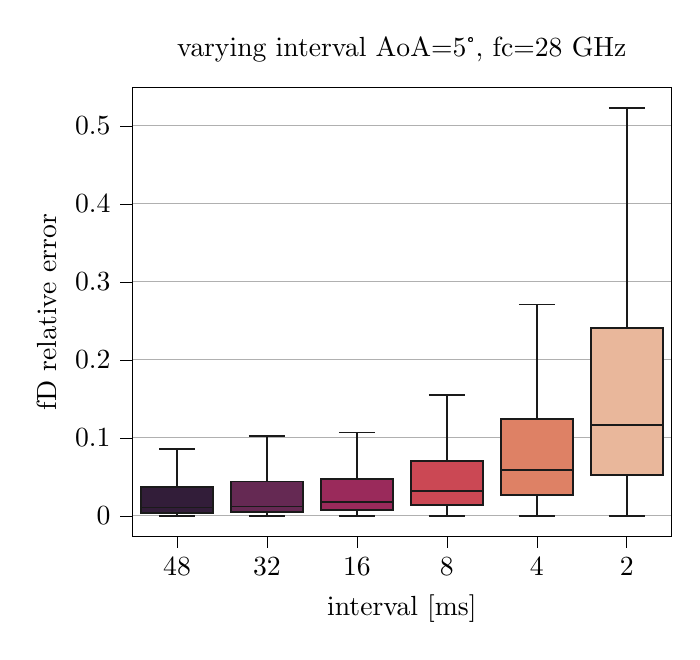
\begin{tikzpicture}

\definecolor{black26}{RGB}{26,26,26}
\definecolor{brown1544291}{RGB}{154,42,91}
\definecolor{burlywood233183155}{RGB}{233,183,155}
\definecolor{darkgray176}{RGB}{176,176,176}
\definecolor{darkslategray1014183}{RGB}{101,41,83}
\definecolor{darkslategray502957}{RGB}{50,29,57}
\definecolor{indianred2037284}{RGB}{203,72,84}
\definecolor{salmon222129101}{RGB}{222,129,101}

\begin{axis}[
tick align=outside,
tick pos=left,
title={varying interval AoA=5°, fc=28 GHz},
x grid style={darkgray176},
xlabel={interval [ms]},
xmin=-0.5, xmax=5.5,
xtick style={color=black},
xtick={0,1,2,3,4,5},
xticklabels={48,32,16,8,4,2},
y grid style={darkgray176},
ylabel={fD relative error},
ymajorgrids,
ymin=-0.0261284808749475, ymax=0.548708570130684,
ytick style={color=black}
]
\path [draw=black26, fill=darkslategray502957, semithick]
(axis cs:-0.4,0.00386707724821807)
--(axis cs:0.4,0.00386707724821807)
--(axis cs:0.4,0.0367560550083486)
--(axis cs:-0.4,0.0367560550083486)
--(axis cs:-0.4,0.00386707724821807)
--cycle;
\path [draw=black26, fill=darkslategray1014183, semithick]
(axis cs:0.6,0.00482911901010105)
--(axis cs:1.4,0.00482911901010105)
--(axis cs:1.4,0.0440217534724169)
--(axis cs:0.6,0.0440217534724169)
--(axis cs:0.6,0.00482911901010105)
--cycle;
\path [draw=black26, fill=brown1544291, semithick]
(axis cs:1.6,0.00773848545304135)
--(axis cs:2.4,0.00773848545304135)
--(axis cs:2.4,0.0474151765949039)
--(axis cs:1.6,0.0474151765949039)
--(axis cs:1.6,0.00773848545304135)
--cycle;
\path [draw=black26, fill=indianred2037284, semithick]
(axis cs:2.6,0.0138977121239652)
--(axis cs:3.4,0.0138977121239652)
--(axis cs:3.4,0.070466680194371)
--(axis cs:2.6,0.070466680194371)
--(axis cs:2.6,0.0138977121239652)
--cycle;
\path [draw=black26, fill=salmon222129101, semithick]
(axis cs:3.6,0.0265021322481822)
--(axis cs:4.4,0.0265021322481822)
--(axis cs:4.4,0.124451280832388)
--(axis cs:3.6,0.124451280832388)
--(axis cs:3.6,0.0265021322481822)
--cycle;
\path [draw=black26, fill=burlywood233183155, semithick]
(axis cs:4.6,0.0519454111816807)
--(axis cs:5.4,0.0519454111816807)
--(axis cs:5.4,0.241141549790301)
--(axis cs:4.6,0.241141549790301)
--(axis cs:4.6,0.0519454111816807)
--cycle;
\addplot [semithick, black26]
table {%
0 0.00386707724821807
0 4.7598894481206e-07
};
\addplot [semithick, black26]
table {%
0 0.0367560550083486
0 0.0859130558628595
};
\addplot [semithick, black26]
table {%
-0.2 4.7598894481206e-07
0.2 4.7598894481206e-07
};
\addplot [semithick, black26]
table {%
-0.2 0.0859130558628595
0.2 0.0859130558628595
};
\addplot [semithick, black26]
table {%
1 0.00482911901010105
1 2.84408498939106e-06
};
\addplot [semithick, black26]
table {%
1 0.0440217534724169
1 0.102479185256538
};
\addplot [semithick, black26]
table {%
0.8 2.84408498939106e-06
1.2 2.84408498939106e-06
};
\addplot [semithick, black26]
table {%
0.8 0.102479185256538
1.2 0.102479185256538
};
\addplot [semithick, black26]
table {%
2 0.00773848545304135
2 4.29836147431566e-06
};
\addplot [semithick, black26]
table {%
2 0.0474151765949039
2 0.106893122468146
};
\addplot [semithick, black26]
table {%
1.8 4.29836147431566e-06
2.2 4.29836147431566e-06
};
\addplot [semithick, black26]
table {%
1.8 0.106893122468146
2.2 0.106893122468146
};
\addplot [semithick, black26]
table {%
3 0.0138977121239652
3 1.0148654730962e-05
};
\addplot [semithick, black26]
table {%
3 0.070466680194371
3 0.155271896489884
};
\addplot [semithick, black26]
table {%
2.8 1.0148654730962e-05
3.2 1.0148654730962e-05
};
\addplot [semithick, black26]
table {%
2.8 0.155271896489884
3.2 0.155271896489884
};
\addplot [semithick, black26]
table {%
4 0.0265021322481822
4 9.71391411633649e-06
};
\addplot [semithick, black26]
table {%
4 0.124451280832388
4 0.271006549119646
};
\addplot [semithick, black26]
table {%
3.8 9.71391411633649e-06
4.2 9.71391411633649e-06
};
\addplot [semithick, black26]
table {%
3.8 0.271006549119646
4.2 0.271006549119646
};
\addplot [semithick, black26]
table {%
5 0.0519454111816807
5 1.10052622602955e-05
};
\addplot [semithick, black26]
table {%
5 0.241141549790301
5 0.522579613266792
};
\addplot [semithick, black26]
table {%
4.8 1.10052622602955e-05
5.2 1.10052622602955e-05
};
\addplot [semithick, black26]
table {%
4.8 0.522579613266792
5.2 0.522579613266792
};
\addplot [semithick, black26]
table {%
-0.4 0.0107000312273137
0.4 0.0107000312273137
};
\addplot [semithick, black26]
table {%
0.6 0.0119001027533172
1.4 0.0119001027533172
};
\addplot [semithick, black26]
table {%
1.6 0.0179499201863071
2.4 0.0179499201863071
};
\addplot [semithick, black26]
table {%
2.6 0.0319735861694599
3.4 0.0319735861694599
};
\addplot [semithick, black26]
table {%
3.6 0.0591136916408563
4.4 0.0591136916408563
};
\addplot [semithick, black26]
table {%
4.6 0.116091837641201
5.4 0.116091837641201
};
\end{axis}

\end{tikzpicture}
